\documentclass[aspectratio=169]{beamer}
\usetheme{Madrid}
\usecolortheme{default}

% Packages
\usepackage{amsmath}
\usepackage{amssymb}
\usepackage{graphicx}
\usepackage{tikz}
\usepackage{booktabs}
\usepackage{xcolor}
\usepackage{listings}

% Title page information
\title[MCDM Implementation]{Multi-Criteria Decision Making for Renewable Energy Planning}
\subtitle{Session 3: Implementation and Practice}
\author{Your Name}
\institute{Your Institution}
\date{\today}

% Custom colors
\definecolor{energygreen}{RGB}{34,139,34}
\definecolor{solarorange}{RGB}{255,140,0}
\definecolor{windblue}{RGB}{70,130,180}
\definecolor{methodred}{RGB}{220,20,60}
\definecolor{toolpurple}{RGB}{128,0,128}

\begin{document}

% Title slide
\begin{frame}
\titlepage
\end{frame}

% Outline
\begin{frame}{Session 3 Overview}
\tableofcontents
\end{frame}

\section{Implementation Framework}

\begin{frame}{MCDM Implementation Framework}
\begin{center}
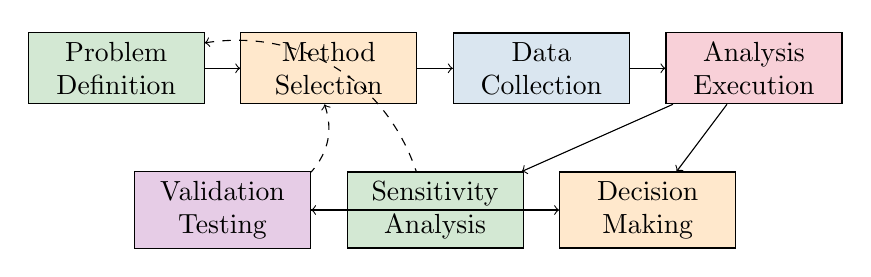
\begin{tikzpicture}[scale=0.9]
% Implementation phases
\node[rectangle, draw, fill=energygreen!20, text width=2cm, align=center] (phase1) at (0,3) {Problem\\Definition};
\node[rectangle, draw, fill=solarorange!20, text width=2cm, align=center] (phase2) at (3,3) {Method\\Selection};
\node[rectangle, draw, fill=windblue!20, text width=2cm, align=center] (phase3) at (6,3) {Data\\Collection};
\node[rectangle, draw, fill=methodred!20, text width=2cm, align=center] (phase4) at (9,3) {Analysis\\Execution};

\node[rectangle, draw, fill=toolpurple!20, text width=2cm, align=center] (phase5) at (1.5,1) {Validation\\Testing};
\node[rectangle, draw, fill=energygreen!20, text width=2cm, align=center] (phase6) at (4.5,1) {Sensitivity\\Analysis};
\node[rectangle, draw, fill=solarorange!20, text width=2cm, align=center] (phase7) at (7.5,1) {Decision\\Making};

% Arrows
\draw[->] (phase1) -- (phase2);
\draw[->] (phase2) -- (phase3);
\draw[->] (phase3) -- (phase4);
\draw[->] (phase4) -- (phase7);
\draw[->] (phase4) -- (phase6);
\draw[->] (phase6) -- (phase5);
\draw[->] (phase5) -- (phase7);

% Feedback loops
\draw[<-, dashed] (phase2) to[bend left=30] (phase5);
\draw[<-, dashed] (phase1) to[bend left=40] (phase6);
\end{tikzpicture}
\end{center}

\textbf{Key Principles:}
\begin{itemize}
\item Iterative process with feedback loops
\item Stakeholder involvement throughout
\item Documentation and transparency
\item Validation and testing at each stage
\end{itemize}
\end{frame>

\begin{frame}{Phase 1: Problem Definition - Best Practices}
\textbf{Critical Questions to Address:}

\begin{columns}
\begin{column}{0.5\textwidth}
\textcolor{energygreen}{\textbf{Context Definition:}}
\begin{itemize}
\item What is the decision context?
\item Who are the stakeholders?
\item What are the constraints?
\item What is the time horizon?
\end{itemize>

\textcolor{solarorange}{\textbf{Scope Boundaries:}}
\begin{itemize}
\item Geographic scope
\item Technology scope
\item Economic scope
\item Environmental scope
\end{itemize>
\end{column>
\begin{column}{0.5\textwidth}
\textcolor{windblue}{\textbf{Success Criteria:}}
\begin{itemize}
\item What constitutes a good decision?
\item How will success be measured?
\item What are the key performance indicators?
\end{itemize>

\textcolor{methodred}{\textbf{Common Pitfalls:}}
\begin{itemize}
\item Unclear objectives
\item Missing stakeholders
\item Unrealistic constraints
\item Scope creep
\end{itemize>
\end{column>
\end{columns>

\vspace{0.3cm}
\textbf{Example:} "Select optimal renewable energy mix for City X to achieve 50\% renewable electricity by 2030 while minimizing costs and maximizing public acceptance."
\end{frame>

\begin{frame}{Phase 2: Method Selection - Decision Tree}
\begin{center}
\begin{tikzpicture}[scale=0.7]
% Decision tree for method selection
\node[rectangle, draw] (start) at (0,0) {Start};

\node[diamond, draw, text width=2cm, align=center] (quant) at (0,-2) {Quantitative\\data only?};
\node[diamond, draw, text width=2cm, align=center] (simple) at (-3,-4) {Simple\\problem?};
\node[diamond, draw, text width=2cm, align=center] (stakeholder) at (3,-4) {High stakeholder\\involvement?};

\node[rectangle, draw, fill=energygreen!20] (saw) at (-5,-6) {SAW};
\node[rectangle, draw, fill=solarorange!20] (wpm) at (-1,-6) {WPM};
\node[rectangle, draw, fill=windblue!20] (topsis) at (1,-6) {TOPSIS};
\node[rectangle, draw, fill=methodred!20] (ahp) at (5,-6) {AHP};

% Connections
\draw[->] (start) -- (quant);
\draw[->] (quant) -- node[left] {Yes} (simple);
\draw[->] (quant) -- node[right] {No} (stakeholder);
\draw[->] (simple) -- node[left] {Yes} (saw);
\draw[->] (simple) -- node[right] {No} (wpm);
\draw[->] (stakeholder) -- node[left] {No} (topsis);
\draw[->] (stakeholder) -- node[right] {Yes} (ahp);
\end{tikzpicture}
\end{center>

\textbf{Additional Considerations:}
\begin{itemize}
\item Available time and resources
\item Software and computational capabilities
\item Team expertise and training needs
\item Regulatory or organizational requirements
\end{itemize>
\end{frame>

\section{Software Tools and Platforms}

\begin{frame}{MCDM Software Landscape}
\begin{columns}
\begin{column}{0.5\textwidth}
\textcolor{energygreen}{\textbf{Free/Open Source:}}
\begin{itemize}
\item \textbf{Excel/Google Sheets}
  \begin{itemize}
  \item Pros: Widely available, customizable
  \item Cons: Manual setup, limited automation
  \end{itemize}
\item \textbf{R (MCDM packages)}
  \begin{itemize}
  \item Pros: Powerful, reproducible
  \item Cons: Programming required
  \end{itemize}
\item \textbf{Python (PyMCDA)}
  \begin{itemize}
  \item Pros: Flexible, extensive libraries
  \item Cons: Coding knowledge needed
  \end{itemize}
\end{itemize>
\end{column>
\begin{column}{0.5\textwidth}
\textcolor{methodred}{\textbf{Commercial Tools:}}
\begin{itemize}
\item \textbf{Expert Choice (AHP)}
  \begin{itemize}
  \item Pros: Professional AHP features
  \item Cons: Expensive, AHP-focused
  \end{itemize}
\item \textbf{1000minds}
  \begin{itemize}
  \item Pros: User-friendly, web-based
  \item Cons: Limited methods
  \end{itemize}
\item \textbf{PROMETHEE-GAIA}
  \begin{itemize}
  \item Pros: Specialized outranking
  \item Cons: Method-specific
  \end{itemize>
\end{itemize>
\end{column>
\end{columns>

\vspace{0.3cm}
\textcolor{toolpurple}{\textbf{Today's Tool:}} Interactive MCDM Learning Platform
\begin{itemize}
\item Web-based, no installation required
\item All four methods (SAW, WPM, TOPSIS, AHP)
\item Built-in renewable energy examples
\item Step-by-step explanations and visualizations
\end{itemize>
\end{frame>

\begin{frame}{Tool Demonstration: MCDM Learning Platform}
\textbf{Live Demonstration Features:}

\begin{columns}
\begin{column}{0.5\textwidth}
\textbf{Data Input:}
\begin{itemize}
\item Example problem selection
\item Custom problem creation
\item CSV import/export
\item Interactive matrix editing
\end{itemize>

\textbf{Analysis:}
\begin{itemize}
\item Method selection
\item Real-time calculations
\item Step-by-step explanations
\item Mathematical formulas (LaTeX)
\end{itemize>
\end{column>
\begin{column}{0.5\textwidth}
\textbf{Results:}
\begin{itemize}
\item Rankings and scores
\item Sensitivity analysis
\item Interactive visualizations
\item Downloadable reports
\end{itemize>

\textbf{Learning:}
\begin{itemize}
\item Method guides
\item Educational resources
\item Example problems
\item Best practices
\end{itemize>
\end{column>
\end{columns>

\vspace{0.3cm}
\textcolor{windblue}{\textbf{URL:}} [Your platform URL here]

\textbf{We'll use this tool for the afternoon group work!}
\end{frame>

\section{Common Pitfalls and Solutions}

\begin{frame}{Common Pitfalls in MCDM Implementation}
\begin{columns}
\begin{column}{0.5\textwidth}
\textcolor{methodred}{\textbf{Pitfall 1: Inconsistent Weighting}}
\begin{itemize}
\item \textbf{Problem:} Weights don't reflect true preferences
\item \textbf{Causes:} Poor elicitation, bias, inconsistency
\item \textbf{Solutions:}
  \begin{itemize}
  \item Use multiple elicitation methods
  \item Check consistency (AHP CR < 0.1)
  \item Involve multiple stakeholders
  \item Perform sensitivity analysis
  \end{itemize>
\end{itemize>

\textcolor{methodred}{\textbf{Pitfall 2: Incomplete Data}}
\begin{itemize}
\item \textbf{Problem:} Missing or unreliable data
\item \textbf{Solutions:}
  \begin{itemize}
  \item Use expert estimates
  \item Interval analysis
  \item Fuzzy numbers
  \item Sensitivity testing
  \end{itemize>
\end{itemize>
\end{column>
\begin{column}{0.5\textwidth}
\textcolor{methodred}{\textbf{Pitfall 3: Method Misapplication}}
\begin{itemize}
\item \textbf{Problem:} Wrong method for the problem type
\item \textbf{Solutions:}
  \begin{itemize}
  \item Follow selection guidelines
  \item Understand method assumptions
  \item Compare multiple methods
  \item Validate with stakeholders
  \end{itemize>
\end{itemize>

\textcolor{methodred}{\textbf{Pitfall 4: Ignoring Uncertainty}}
\begin{itemize}
\item \textbf{Problem:} Treating uncertain data as precise
\item \textbf{Solutions:}
  \begin{itemize}
  \item Monte Carlo simulation
  \item Scenario analysis
  \item Robust optimization
  \item Confidence intervals
  \end{itemize>
\end{itemize>
\end{column>
\end{columns>
\end{frame>

\begin{frame}{Quality Assurance Checklist}
\textbf{Before Implementation:}
\begin{itemize}
\item ✓ Clear problem definition and objectives
\item ✓ Complete stakeholder identification
\item ✓ Appropriate method selection
\item ✓ Data quality assessment
\end{itemize>

\textbf{During Implementation:}
\begin{itemize}
\item ✓ Consistent data collection procedures
\item ✓ Regular stakeholder validation
\item ✓ Documentation of assumptions
\item ✓ Intermediate result checking
\end{itemize>

\textbf{After Implementation:}
\begin{itemize}
\item ✓ Sensitivity analysis performed
\item ✓ Results validated with stakeholders
\item ✓ Limitations clearly stated
\item ✓ Implementation plan developed
\end{itemize>

\textcolor{energygreen}{\textbf{Remember:}} MCDM is a decision support tool, not a decision replacement!
\end{frame>

\section{Group Work Preparation}

\begin{frame}{Afternoon Group Work: Detailed Instructions}
\textbf{Group Formation:} 6 groups, 4-5 people each

\textbf{Problem Assignment:}
\begin{enumerate}
\item \textcolor{energygreen}{\textbf{Group 1:}} Regional Energy Planning (City scale)
\item \textcolor{solarorange}{\textbf{Group 2:}} Campus Energy Planning (University)
\item \textcolor{windblue}{\textbf{Group 3:}} Rural Electrification Planning
\item \textcolor{methodred}{\textbf{Group 4:}} Industrial Energy Selection
\item \textcolor{toolpurple}{\textbf{Group 5:}} Residential Energy Systems
\item \textcolor{gray}{\textbf{Group 6:}} Community Energy Projects
\end{enumerate>

\textbf{Time Allocation:}
\begin{itemize}
\item 13:00-13:30: Group formation and problem exploration
\item 13:30-15:00: MCDM analysis and calculations
\item 15:00-15:15: Coffee break
\item 15:15-16:30: Sensitivity analysis and report preparation
\item 16:30-17:00: Group presentations (5 min each + Q\&A)
\end{itemize>
\end{frame>

\begin{frame}{Group Work Tasks and Deliverables}
\textbf{Required Tasks:}
\begin{enumerate}
\item \textbf{Problem Analysis} (30 min)
  \begin{itemize}
  \item Define decision context and stakeholders
  \item Identify alternatives and criteria
  \item Discuss weighting approach
  \end{itemize>

\item \textbf{MCDM Application} (90 min)
  \begin{itemize}
  \item Apply at least 2 different methods
  \item Document assumptions and data sources
  \item Calculate results using the platform
  \end{itemize>

\item \textbf{Analysis and Validation} (75 min)
  \begin{itemize}
  \item Perform sensitivity analysis
  \item Compare method results
  \item Validate with group consensus
  \end{itemize>
\end{enumerate>

\textbf{Deliverables:}
\begin{itemize}
\item 5-minute presentation
\item Completed analysis (downloadable from platform)
\item Key insights and recommendations
\end{itemize>
\end{frame>

\begin{frame}{Group Work: Problem Descriptions}
\begin{columns}
\begin{column}{0.5\textwidth}
\textbf{Regional Energy Planning:}
\begin{itemize}
\item City of 500k people
\item 40\% demand increase by 2035
\item 8 energy alternatives
\item 7 evaluation criteria
\end{itemize>

\textbf{Campus Energy Planning:}
\begin{itemize}
\item University with 15k students
\item \$2.5M annual electricity cost
\item Carbon neutrality by 2030
\item 5 energy solutions
\end{itemize>

\textbf{Rural Electrification:}
\begin{itemize}
\item 50k residents, 30\% grid access
\item Development funding available
\item 6 electrification options
\item Social impact focus
\end{itemize>
\end{column>
\begin{column}{0.5\textwidth}
\textbf{Industrial Energy:}
\begin{itemize}
\item Manufacturing facility
\item High energy demand (24/7)
\item Cost and reliability critical
\item 5 energy alternatives
\end{itemize>

\textbf{Residential Energy:}
\begin{itemize}
\item Suburban neighborhood
\item 200 households
\item Individual vs. community systems
\item 6 technology options
\end{itemize>

\textbf{Community Energy:}
\begin{itemize}
\item Local energy cooperative
\item Community ownership model
\item Environmental priorities
\item 5 renewable options
\end{itemize>
\end{column>
\end{columns>

\textcolor{blue}{\textbf{All problems include:}} Pre-loaded data, criteria definitions, and guidance materials
\end{frame>

\begin{frame}{Presentation Guidelines}
\textbf{Presentation Structure (5 minutes):}
\begin{enumerate}
\item \textbf{Problem Context} (1 min)
  \begin{itemize}
  \item Brief problem description
  \item Key stakeholders and constraints
  \end{itemize>

\item \textbf{MCDM Approach} (2 min)
  \begin{itemize}
  \item Methods used and rationale
  \item Criteria and weights
  \item Key assumptions
  \end{itemize>

\item \textbf{Results and Insights} (2 min)
  \begin{itemize}
  \item Ranking results
  \item Sensitivity analysis findings
  \item Method comparison
  \item Final recommendation
  \end{itemize>
\end{enumerate>

\textbf{Evaluation Criteria:}
\begin{itemize}
\item Clarity of problem definition
\item Appropriateness of method selection
\item Quality of analysis and validation
\item Practical relevance of recommendations
\end{itemize>
\end{frame>

\section{Course Summary and Next Steps}

\begin{frame}{Three-Session Journey Summary}
\textbf{Session 1: Fundamentals}
\begin{itemize}
\item MCDM concepts and components
\item Renewable energy decision challenges
\item Five-step MCDM process
\end{itemize>

\textbf{Session 2: Methods}
\begin{itemize}
\item SAW, WPM, TOPSIS, AHP
\item Method comparison and selection
\item Case study applications
\end{itemize>

\textbf{Session 3: Implementation}
\begin{itemize}
\item Implementation framework
\item Software tools and platforms
\item Common pitfalls and solutions
\item Hands-on group work
\end{itemize>

\vspace{0.3cm}
\textcolor{energygreen}{\textbf{Key Achievement:}} You now have practical skills to apply MCDM to real renewable energy decisions!
\end{frame>

\begin{frame}{Beyond This Course: Next Steps}
\textbf{Immediate Applications:}
\begin{itemize}
\item Apply MCDM to your research projects
\item Use the learning platform for practice
\item Explore additional example problems
\item Share knowledge with colleagues
\end{itemize>

\textbf{Advanced Learning:}
\begin{itemize}
\item Study advanced MCDM methods (ELECTRE, PROMETHEE)
\item Learn fuzzy MCDM for uncertainty handling
\item Explore group decision making techniques
\item Investigate multi-objective optimization
\end{itemize>

\textbf{Professional Development:}
\begin{itemize}
\item Join MCDM research communities
\item Attend specialized conferences
\item Collaborate on energy planning projects
\item Develop domain expertise
\end{itemize>

\textbf{Resources:} Learning platform includes extensive bibliography and links to advanced materials
\end{frame>

\begin{frame}{Final Thoughts: MCDM for Sustainable Energy}
\begin{block}{The Challenge}
Renewable energy decisions are among the most complex and important decisions of our time, involving multiple stakeholders, long-term commitments, and significant uncertainties.
\end{block>

\begin{block}{The Opportunity}
MCDM provides a systematic, transparent, and scientifically sound approach to navigate this complexity and make better decisions for a sustainable energy future.
\end{block>

\textbf{Remember:}
\begin{itemize}
\item MCDM is a tool to support, not replace, human judgment
\item The process is often as valuable as the results
\item Stakeholder involvement is crucial for success
\item Continuous learning and adaptation are essential
\end{itemize>

\vspace{0.3cm}
\begin{center}
\textcolor{energygreen}{\Large Good luck with your group work!}\\
\textcolor{windblue}{\Large Questions before we begin?}
\end{center>
\end{frame>

\end{document>
